%% Closed-loop cold atmospheric plasma delivery with embedded sensing
%% Elsevier review article (elsarticle, author-year). Build: latexmk -pdf main.tex
\documentclass[preprint,review,12pt,authoryear]{elsarticle}

\usepackage[T1]{fontenc}
\usepackage{lmodern}
\usepackage{amsmath,amssymb}
\usepackage{graphicx}
\usepackage{booktabs}
\usepackage{tabularx}
\usepackage{array}
\usepackage{siunitx}
\usepackage[version=4]{mhchem}
\usepackage{lineno}
\usepackage[hidelinks]{hyperref}
\usepackage{doi}

\graphicspath{{figures/}}
\newcolumntype{L}{>{\raggedright\arraybackslash}X}
\sisetup{detect-all}
\modulolinenumbers[5]
\linenumbers

\journal{Biosensors and Bioelectronics}

% Drop the "Preprint submitted to" footer, which collides with the author footnote.
\makeatletter
\def\ps@pprintTitle{\let\@oddhead\@empty\let\@evenhead\@empty
  \let\@oddfoot\@empty\let\@evenfoot\@empty}
\makeatother

\begin{document}

\begin{frontmatter}

\title{Closed-loop cold atmospheric plasma delivery with embedded sensing: a critical review of sensing, control and integration, with an in-silico analysis of where dose error originates}

\author{M. Nisha Angeline\corref{cor1}}
\ead{nishavlsidesign@gmail.com}
\cortext[cor1]{Corresponding author. ORCID: [to be added].}
\affiliation{organization={Department of Electronics and Communication Engineering, Velalar College of Engineering and Technology},
            addressline={Thindal},
            city={Erode},
            postcode={638012},
            state={Tamil Nadu},
            country={India}}

\begin{abstract}
Cold atmospheric plasma (CAP) is delivered almost everywhere in open loop: an operator fixes voltage, gas flow, stand-off distance and time, and the delivered dose varies with tissue, geometry and ambient conditions. Closed-loop delivery, in which on-device sensing drives a controller that adjusts the plasma source, has been proposed to make CAP reproducible and safe, but its building blocks have matured unevenly. We critically review four layers of a closed-loop CAP system: embedded sensing (electrochemical, optical-emission and electrical), state estimation and dosimetry, feedback control (model predictive, adaptive and learning-based), and actuation and integration hardware, using adjacent closed-loop therapies (insulin, anaesthesia, drug delivery) as translational benchmarks. Every reference was audited for existence and claim support. The literature shows that constraint-aware model predictive control can already hold CAP thermal dose within safety limits, whereas sensors for reactive species drift, foul and lose selectivity under plasma exposure, and few devices co-integrate sensing, control and actuation. An illustrative Monte Carlo case study on a generic lumped thermal model (1000 virtual treatments per arm) quantifies this asymmetry: feedback reduced the median absolute CEM43 thermal-dose error from 89\% to 17\% and safety-limit violations from 32\% to 0.1\% of treatments, but the residual error tracked sensor bias and lag rather than plant variation, and a degraded sensor raised it to 50\%. We conclude with six benchmark metrics and a staged roadmap from sensor-supervised to fully closed-loop CAP.
\end{abstract}

\begin{highlights}
\item Closed-loop cold plasma delivery is limited by sensing, not by control theory.
\item Constrained MPC already regulates CAP thermal dose under safety limits.
\item In-silico: feedback cuts median thermal-dose error from 89\% to 17\%.
\item Residual closed-loop error is set by sensor bias and lag, not plant variation.
\item We propose six benchmark metrics for reporting closed-loop CAP devices.
\end{highlights}

\begin{keyword}
cold atmospheric plasma \sep closed-loop control \sep embedded biosensing \sep model predictive control \sep plasma dosimetry \sep reactive oxygen and nitrogen species \sep medical devices
\end{keyword}

\end{frontmatter}

%% ---------------------------------------------------------------------------
\section{Introduction}
\label{sec:intro}

Cold atmospheric plasma (CAP) is a partially ionised gas near room temperature that delivers reactive oxygen and nitrogen species (RONS), electric fields, ultraviolet photons and modest heat to a target. Randomised trials in chronic wounds \citep{isbary2010,brehmer2015,strohal2022} and a large preclinical literature in wound healing and oncology \citep{schmidt2019,he2020,dubuc2018} have established CAP as a credible redox-based therapy \citep{vonwoedtke2019,laroussi2020}.

Yet CAP is almost always delivered in open loop. The operator selects voltage, frequency, gas flow, stand-off distance and treatment time, and the delivered dose follows from physics the device does not observe. Dose depends on source design, feed gas, target conductivity and moisture, geometry and ambient humidity \citep{dai2020,miebach2022}, so identical settings do not guarantee identical effects. No universal definition of plasma dose exists, and reviews repeatedly name dosimetry and reproducibility as the main barriers to clinical translation \citep{dai2020,boehm2018}.

Closed-loop delivery addresses this by measuring a treatment-relevant state during exposure and adjusting the source to hold that state, or its time integral, within a target window \citep{bonzanini2022}. Closed-loop control has transformed other therapies: hybrid closed-loop insulin delivery increases time in target range in randomised trials \citep{ware2022}, and automated anaesthetic delivery improves time within the target depth \citep{felippe2026}. For CAP, the components exist in separate literatures: in situ electrochemical sensors for RONS \citep{nasri2021,thomas2026a}, optical and electrical plasma-state sensing \citep{chan2025} and constrained model predictive control of plasma jets \citep{gidon2017}. They have rarely been combined in one device (Fig.~\ref{fig:arch}).

\begin{figure}[t]
\centering
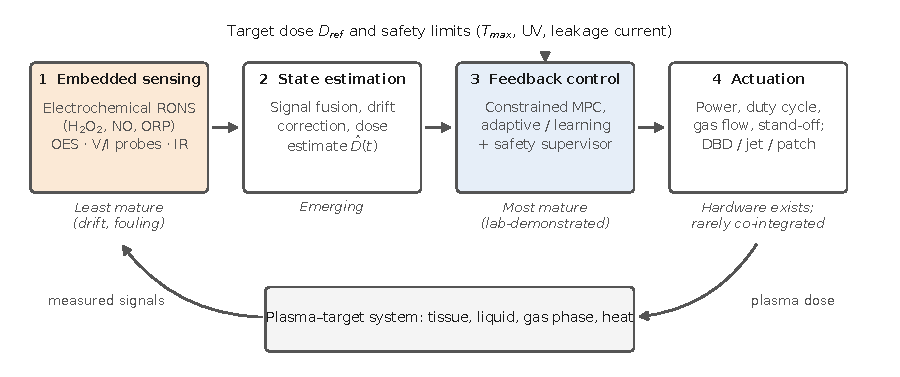
\includegraphics[width=\textwidth]{Fig1_architecture.pdf}
\caption{Four-layer architecture of a closed-loop CAP system. Shading marks the least mature layer (sensing, orange) and the most mature layer (control, blue), as graded in Sections~\ref{sec:sensing}--\ref{sec:hardware}.}
\label{fig:arch}
\end{figure}

\subsection{Contributions}

This review makes four contributions beyond existing reviews of CAP dosimetry and wearable CAP devices:
\begin{enumerate}
\item It organises closed-loop CAP into four layers (sensing, state estimation, control, actuation) and grades the maturity of each against the same evidence criteria (Sections~\ref{sec:dose}--\ref{sec:hardware}).
\item It quantifies, with a reproducible Monte Carlo case study, how much feedback helps and where the residual error comes from, showing that sensor bias and lag, not plant variability, set the floor (Section~\ref{sec:case}).
\item It proposes six benchmark metrics that would make closed-loop CAP devices comparable across laboratories (Section~\ref{sec:safety}).
\item It documents the reference-integrity screening applied to the evidence base, including the criteria for removing sources (Section~\ref{sec:method}).
\end{enumerate}
Section~\ref{sec:method} describes the review method. Sections~\ref{sec:dose}--\ref{sec:hardware} cover the four layers, Section~\ref{sec:case} the case study, Section~\ref{sec:safety} safety, standardisation and metrics, and Section~\ref{sec:roadmap} a roadmap and conclusions.

%% ---------------------------------------------------------------------------
\section{Review methodology}
\label{sec:method}

This is a critical narrative review, not a PRISMA systematic review; it does not claim exhaustive retrieval or perform meta-analysis.

\paragraph{Evidence identification} An initial evidence map (87 records) was generated with an AI-assisted literature tool (LeapSpace, Elsevier) querying Scopus-indexed literature on CAP sensing, plasma diagnostics, plasma control, CAP hardware and closed-loop biomedical delivery, with emphasis on 2018--2026. Targeted primary sources (e.g., the CEM43 thermal-dose definition, DIN SPEC 91315 and primary closed-loop drug-delivery studies) were then added to fill gaps.

\paragraph{Integrity screening} Every record was checked for (i) existence and correct bibliographic metadata via its DOI, and (ii) whether its content supports the specific claim for which it is cited. Records were removed when they could not be verified, were off-topic (e.g., aerodynamic flow-control actuators, fire-evacuation guidance, food-delivery logistics), or were secondary sources where a primary study was available. Of the 87 records, 42 were retained, 19 were removed (10 off-topic, 1 duplicate, 1 secondary, 5 not supporting the cited claim, 2 unidentifiable), 26 were relevant but not needed, and 8 verified primary sources were added, giving 50 references.

\paragraph{Inclusion criteria} Retained studies address at least one of: real-time measurement of CAP-relevant species, plasma state or tissue response; feedback or model-based control of atmospheric-pressure plasma sources; integrated or wearable CAP hardware; closed-loop biomedical delivery with a quantitative open- versus closed-loop comparison; or CAP safety and dosimetry standards.

\paragraph{Evidence grading} Each conclusion in Sections~\ref{sec:dose}--\ref{sec:hardware} carries one of three grades (Table~\ref{tab:grades}).

\begin{table}[h]
\centering
\caption{Evidence grades used in this review.}
\label{tab:grades}
\begin{tabularx}{\textwidth}{@{}lL@{}}
\toprule
Grade & Meaning \\
\midrule
A & Demonstrated experimentally in a CAP system, in more than one independent study \\
B & Demonstrated in a single CAP study, in simulation, or in an adjacent closed-loop domain \\
C & Inference by the author from indirect evidence; stated as a hypothesis \\
\bottomrule
\end{tabularx}
\end{table}

%% ---------------------------------------------------------------------------
\section{What must be controlled: CAP dose as a multiphysics state}
\label{sec:dose}

CAP dose is not one observable quantity, so a closed-loop controller must regulate a proxy, or an estimate built from several proxies. The biological effect depends on coupled electrical input, reactive-species generation, gas-phase and liquid-phase transport, heat load and the target's response \citep{dai2020}. Four candidate controlled variables appear in the literature, in decreasing order of measurability (Table~\ref{tab:cv}).

\begin{table}[h]
\centering
\caption{Candidate controlled variables for closed-loop CAP.}
\label{tab:cv}
\small
\begin{tabularx}{\textwidth}{@{}LLlL@{}}
\toprule
Controlled variable & Typical sensor & Closeness to effect & Maturity \\
\midrule
Surface temperature and cumulative thermal dose & IR thermometry, thermocouple & Low (safety) & A: regulated in closed loop \citep{gidon2017,gidon2021} \\
Plasma state (emission intensity, current, power) & OES, voltage and current probes & Medium & B: sensed and classified in real time \citep{chan2025} \\
Delivered RONS (\ce{H2O2}, \ce{NO2-}, NO, ORP, pH) & Electrochemical micro-electrodes & High & B: monitored in situ, not yet closed loop \citep{nasri2021,thomas2026a} \\
Tissue response (oxygenation, microcirculation) & Optical spectroscopy, microfluidic biosensing & Highest & C for control; measured serially \citep{kisch2016a} \\
\bottomrule
\end{tabularx}
\end{table}

The trade-off is plain: the variables easiest to sense are furthest from efficacy. Thermal dose is the one variable already controlled in closed loop, because temperature is cheap to measure and its biological integral is well defined. Cumulative equivalent minutes at \SI{43}{\celsius} (CEM43) is computed from the temperature history \citep{sapareto1984}:
\begin{equation}
\mathrm{CEM43} = \int_0^{t_f} R^{\,43 - T(t)}\, \mathrm{d}t, \qquad
R = \begin{cases} 0.5, & T \ge 43\,^{\circ}\mathrm{C}, \\ 0.25, & T < 43\,^{\circ}\mathrm{C}. \end{cases}
\label{eq:cem43}
\end{equation}
\citet{gidon2017} generalised this integral form to a cumulative, non-decreasing plasma dose metric, which is the structure a controller needs: a monotone quantity that ends the treatment once it reaches a target. A RONS-based dose could take the same form if a sensor delivered a calibrated, drift-free species flux, which is the gap examined in Section~\ref{sec:sensing}.

In short, a closed-loop CAP system needs four layers: sensing, state estimation that maps signals to a dose estimate, a control policy that respects safety constraints, and an actuator that responds predictably to commands \citep{bonzanini2022}.

%% ---------------------------------------------------------------------------
\section{Embedded sensing modalities}
\label{sec:sensing}

Sensing is the least mature layer of closed-loop CAP: species-specific sensors exist and work in situ, but none yet combines selectivity, stability under repeated plasma exposure and calibration traceability (Grade A for the bottleneck itself).

\subsection{Electrochemical sensing of reactive species and redox state}

Electrochemical sensors read chemically meaningful variables at the treatment site, which makes them the most direct route to an efficacy-related controlled variable. \citet{nasri2021} built an electrochemical sensor for in situ monitoring of reactive species produced by cold physical plasma and proposed it explicitly as a means to control species delivery. \citet{thomas2026a} monitored \ce{H2O2} and oxidation--reduction potential (ORP) during CAP therapy; both rose with plasma dose and correlated with wound-healing outcomes, an association the authors present as correlational rather than causal. Multiparametric platforms with \ce{H2O2}, nitrite/NO and lactate channels have been demonstrated for continuous monitoring outside plasma settings \citep{chmayssem2021}. These studies stop at monitoring or post hoc correlation; none closes the loop to the plasma source (Grade B).

\subsection{Optical and electrical plasma-state sensing}

Optical emission spectroscopy (OES) identifies excited species (OH, the \ce{N2} second positive system, NO-$\gamma$, atomic O) and yields rotational and vibrational temperatures \citep{machala2007}. \citet{chan2025} combined real-time OES with discharge voltage and current probes and used machine learning to distinguish ex vivo biological tissues during treatment, turning the plasma itself into a sensor of what it touches. Electrical signals are fast, cheap and unaffected by fouling, which suits inner control loops, whereas optical channels add species information at higher cost.

The design principle that follows is multimodal state estimation: chemical, optical and electrical channels have complementary bandwidths and failure modes, and fusing them should give a better dose estimate than any single channel (Grade C).

\subsection{Drift, fouling, selectivity and lifetime}

Sensor durability is the binding constraint. Continuous electrochemical biosensors suffer baseline drift, biofouling and receptor degradation in complex media; mitigations include antifouling coatings, reference channels and ratiometric or dual-frequency read-outs \citep{kimg2026}. Under CAP the problem is sharper, because the oxidants the sensor measures also attack its surface. \citet{thomas2026b} examined NO and \ce{Ca^2+} sensors during CAP treatment of acute wounds and found that the NO sensor degraded within about one hour of plasma exposure, with selectivity limited in the plasma--bio environment. Table~\ref{tab:modality} summarises the modalities. The case study in Section~\ref{sec:case} shows why this matters quantitatively: once feedback removes plant variability, sensor bias and lag become the dominant source of dose error.

\begin{table}[h]
\centering
\caption{Sensing modalities for closed-loop CAP.}
\label{tab:modality}
\small
\begin{tabularx}{\textwidth}{@{}LLlLL@{}}
\toprule
Modality & Measured & Bandwidth & Main failure mode & Closed-loop CAP shown? \\
\midrule
Electrochemical (amperometric, potentiometric) & \ce{H2O2}, NO, \ce{NO2-}, ORP, pH & Seconds & Fouling, oxidant attack, drift & No (monitoring only) \\
Optical emission spectroscopy & Excited species, gas temperature & Milliseconds & Calibration, line of sight, cost & Intensity regulated \citep{gidon2021} \\
Electrical probes & Voltage, current, power & Microseconds & Indirect link to dose & Classification \citep{chan2025} \\
Infrared thermometry & Surface temperature & Sub-second & Emissivity bias & Yes \citep{gidon2017} \\
\bottomrule
\end{tabularx}
\end{table}

%% ---------------------------------------------------------------------------
\section{Feedback control strategies}
\label{sec:control}

Control is the most mature layer: constrained model predictive control (MPC) has regulated CAP thermal dose and plasma intensity experimentally while enforcing safety limits (Grade A for thermal and intensity outputs).

\subsection{Model predictive and constraint-aware control}

MPC suits CAP because it handles hard constraints (maximum surface temperature, power limits) and cumulative targets explicitly. \citet{gidon2016} used MPC with successive linearisation of a nonlinear thermal model to deliver a predetermined thermal dose from an atmospheric-pressure plasma jet (APPJ) without exceeding a temperature limit. \citet{gidon2017} extended this to a cumulative plasma dose metric with a safe operating region and showed better disturbance rejection than PI control in simulation. \citet{gidon2021} identified a linear parameter-varying (LPV) model from data and demonstrated hierarchical LPV-MPC experimentally, regulating the surface temperature and optical intensity of a CAP jet and the spatial delivery of cumulative thermal effects. A general constrained MPC formulation for CAP dose delivery is
\begin{equation}
\begin{aligned}
\min_{u_{0:N-1}} \quad & \sum_{k=0}^{N-1} \bigl\| D_{\mathrm{ref}} - \hat{D}_{k} \bigr\|_{Q}^{2} + \bigl\| \Delta u_k \bigr\|_{R}^{2} \\
\text{s.t.} \quad & x_{k+1} = f(x_k, u_k), \quad T_k \le T_{\max}, \quad u_{\min} \le u_k \le u_{\max},
\end{aligned}
\label{eq:mpc}
\end{equation}
where $u$ is the actuator vector (applied power, duty cycle, gas flow or stand-off), $x$ the estimated plasma--target state, $\hat{D}$ the estimated cumulative dose and $T$ the surface temperature.

\subsection{Adaptive and robust control}

Model mismatch is unavoidable because tissue properties change between patients and within a treatment. \citet{rodrigues2023} applied data-driven modifier adaptation to estimate plant--model mismatch in both cost and constraints for CAP, reaching a cumulative thermal-effect target while tracking path constraints. \citet{ghafghanbari2024} proposed adaptive robust LPV-MPC for APPJs and reported improved tracking under modelling errors and disturbances (Grade B; conference study).

\subsection{Learning-based control}

Machine learning has been proposed throughout the CAP control stack, from tissue identification to approximate MPC that fits on embedded hardware \citep{bonzanini2022}. Learning-based stochastic MPC has tracked a reference thermal dose on an APPJ while respecting a temperature constraint \citep{bonzanini2021}, and fast deep-learning MPC policies have been adapted to new targets with little data \citep{chan2023}. Experimentally validated reinforcement-learning controllers for biomedical CAP were not found in the audited evidence (Grade C for any advantage over MPC). The safe path is learning inside a constraint-enforcing envelope: a learned model or policy proposes, and a verified supervisory layer enforces temperature and dose limits.

\subsection{Benchmarks from adjacent closed-loop therapies}

Closed-loop delivery improves precision in every adjacent domain with randomised evidence. In critically ill adults, fully automated closed-loop glucose control raised time in target range to 54.3\% versus 18.5\% with standard care \citep{leelarathna2013}. In children and adolescents with type~1 diabetes, the Cambridge hybrid closed-loop algorithm increased time in range over six months \citep{ware2022}, and automated hypnotic delivery during anaesthesia improved time within the target depth in meta-analysis \citep{felippe2026}. In live animals, closed-loop control regulated circulating doxorubicin concentration in real time using an aptamer-based sensor \citep{mage2017}. No study has yet compared closed-loop and open-loop CAP in the same device and model (Grade C for the size of the benefit); Section~\ref{sec:case} estimates it in silico.

%% ---------------------------------------------------------------------------
\section{Actuation and integration hardware}
\label{sec:hardware}

CAP actuators already exist in portable and flexible formats, but the sensor--controller--actuator stack is rarely co-integrated: most devices still rely on benchtop oscilloscopes, probes and spectrometers (Grade A).

\subsection{Source architectures}

Dielectric barrier discharges (DBDs), plasma jets and flexible surface-DBD patches dominate biomedical CAP \citep{lu2021,emmert2013}. Wearable flexible CAP devices built on printed circuits and compact high-voltage supplies have been reviewed recently; the same review notes that they still lack power autonomy, real-time sensing and adaptive control \citep{zhang2026}. Device-design studies typically keep diagnostics external to the source \citep{quintero2025}.

\subsection{Actuation variables}

Each source parameter shifts dose along a different axis. Feed gas sets chemistry: air DBDs favour ozone and nitrogen oxides, whereas noble-gas jets favour short-lived OH and atomic oxygen \citep{machala2007,lu2021}. Applied voltage, frequency, pulse shape and duty cycle set power and heat \citep{kimyw2003}. Target conductivity changes the current path and RONS delivery \citep{miebach2022}, and electrode--tissue contact area changes the physical parameters of DBD wound sources \citep{borchardt2025}. Of these, duty cycle and applied power are the natural fast actuators for feedback; gas composition and geometry are better treated as slow set-points.

\subsection{Plasma-activated carriers as a decoupled actuator}

Plasma-activated liquids and hydrogels store plasma-derived species and release them over time, which separates generation from delivery \citep{biazar2024,kuddushi2026}. Species formation in activated liquids depends on discharge conditions and on the liquid itself \citep{bae2026}. Decoupling may make carriers easier to regulate than direct jets, because loading can be measured before application, but no closed-loop CAP carrier was found in the audited literature (Grade C).

\subsection{Integration templates from adjacent devices}

Adjacent devices show how to integrate sensing, control and actuation in small form factors: a battery-free, NFC-powered wound dressing that monitors infection and releases drug on demand \citep{xu2021}, a wireless battery-free implant for closed-loop neuromodulation \citep{ouyang2023}, a soft implant controlled wirelessly by a wearable \citep{joo2021} and a wirelessly controlled drug-delivery microchip tested in humans \citep{farra2012}. A CAP equivalent must also isolate kilovolt drive electronics from low-noise sensor front-ends, a constraint none of these templates faces.

%% ---------------------------------------------------------------------------
\section{Illustrative in-silico case study: where closed-loop dose error comes from}
\label{sec:case}

Feedback removes the dose error caused by plant variability but leaves an error floor set by the sensor. This section quantifies that claim on a deliberately simple model; it illustrates mechanisms and does not predict the performance of any specific device.

\subsection{Model}

Surface temperature $T$ under a CAP jet was modelled as a first-order lumped system driven by applied power $P$, a standard simplification of the APPJ thermal models used in CAP control studies \citep{gidon2016}:
\begin{equation}
\tau \frac{\mathrm{d}T}{\mathrm{d}t} = -\bigl(T - T_{\mathrm{amb}}\bigr) + K\,P(t), \qquad 0 \le P \le P_{\max}.
\label{eq:plant}
\end{equation}
Nominal parameters were $T_{\mathrm{amb}} = \SI{32}{\celsius}$, $\tau = \SI{8}{\second}$, $K = \SI{3}{\celsius\per\watt}$ and $P_{\max} = \SI{5}{\watt}$ (illustrative values chosen to give clinically plausible surface temperatures, not fitted to data). The treatment target was CEM43 $= \SI{1.0}{\minute}$ with a hard safety limit $T \le \SI{45}{\celsius}$. Each virtual treatment drew $K$ from $\mathcal{U}(0.75, 1.25)\times$ nominal (stand-off and gas-flow variation), $\tau$ from $\mathcal{U}(0.8, 1.2)\times$ nominal (tissue thermal properties) and $T_{\mathrm{amb}}$ from $\mathcal{N}(32, 1)$\,\si{\celsius}. Equations~\eqref{eq:cem43} and \eqref{eq:plant} were integrated with forward Euler at $\Delta t = \SI{0.1}{\second}$; 1000 treatments were simulated per arm on the same set of plants.

\subsection{Delivery strategies}

\begin{itemize}
\item \textbf{Open loop:} constant power calibrated to a \SI{44}{\celsius} steady state on the nominal plant (\SI{4.0}{\watt}), applied for the time that delivers the target dose on that plant (\SI{52.6}{\second}).
\item \textbf{Closed loop, nominal sensor:} PI temperature control ($k_p = \SI{1.2}{\watt\per\celsius}$, $k_i = \SI{0.15}{\watt\per\celsius\per\second}$) at a \SI{44}{\celsius} set-point with conditional-integration anti-windup and a supervisory interlock at \SI{44.7}{\celsius}; treatment ends when CEM43 estimated from the measured temperature reaches the target. Sensor: \SI{1}{\second} first-order lag, Gaussian noise $\sigma = \SI{0.2}{\celsius}$ and a per-treatment calibration bias drawn from $\mathcal{N}(0, 0.3)$\,\si{\celsius}.
\item \textbf{Closed loop, degraded sensor:} the same controller with a \SI{3}{\second} lag, $\sigma = \SI{0.5}{\celsius}$ noise and $\mathcal{N}(0, 1.0)$\,\si{\celsius} bias, representing fouling or emissivity error.
\end{itemize}

\subsection{Results}

Open-loop error depends almost entirely on how far the plant departs from calibration, because CEM43 grows exponentially with temperature: in the highest gain bin the median delivered dose was 4.5 times the target (Fig.~\ref{fig:dose}). Closed-loop medians stay within a few percent of target across the whole gain range, so feedback has removed the plant dependence; what remains is a spread that does not change with gain and widens sharply when the sensor degrades (Table~\ref{tab:results}).

\begin{figure}[t]
\centering
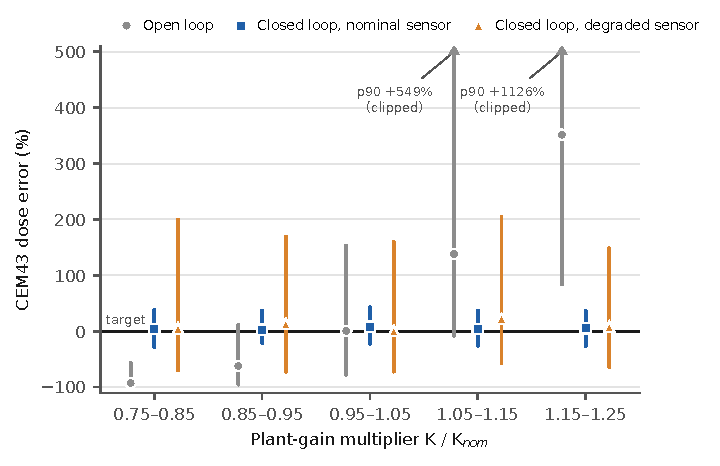
\includegraphics[width=0.75\textwidth]{Fig2_dose_error.pdf}
\caption{CEM43 dose error by plant-gain bin for the three delivery strategies (point: median; whisker: 10th--90th percentile; open-loop whiskers above +500\% are clipped and labelled). Monte Carlo simulation by the author (seed 2026, 1000 treatments per arm) on a generic lumped thermal model not fitted to any device.}
\label{fig:dose}
\end{figure}

\begin{table}[h]
\centering
\caption{In-silico case study results (1000 treatments per arm). Dose error is computed from the true temperature; safety exceedance is any true temperature above \SI{45}{\celsius}.}
\label{tab:results}
\small
\begin{tabularx}{\textwidth}{@{}Lcccc@{}}
\toprule
Strategy & Median $|$dose error$|$ & Within $\pm$10\% & Exceeding \SI{45}{\celsius} & Median time \\
\midrule
Open loop & 89\% & 5.9\% & 31.5\% & \SI{52.6}{\second} (fixed) \\
Closed loop, nominal sensor & 17\% & 33.9\% & 0.1\% & \SI{49.0}{\second} \\
Closed loop, degraded sensor & 50\% & 11.3\% & 13.9\% & \SI{52.3}{\second} \\
\bottomrule
\end{tabularx}
\end{table}

\subsection{Interpretation and limitations}

Two results carry over to real devices. First, because thermal dose is exponential in temperature, a calibration bias of a few tenths of a degree produces tens of percent of dose error, which is why metric M5 (sensor drift budget, Section~\ref{sec:metrics}) matters. Second, the degraded sensor re-introduced safety violations in 13.9\% of treatments despite the interlock, because a biased sensor hides the true temperature from the supervisor.

The model omits spatial heat spread, RONS chemistry, controller optimisation and MPC; a tuned MPC with a state estimator would reduce the spread but cannot remove an unobserved bias. Results are illustrative and should not be cited as device performance. The Python script and its full numerical output are provided as Supplementary Material S1 (deterministic, seed 2026).

%% ---------------------------------------------------------------------------
\section{Safety, standardisation and proposed benchmark metrics}
\label{sec:safety}

Closed-loop CAP cannot be compared across laboratories today, because no study reports dose error, time in target, latency or fault behaviour in a common form. We propose six metrics to fix this.

\subsection{Safety benchmarks}

DIN SPEC 91315:2014 \citep{dinspec91315}, since withdrawn with a revision project under way, set general requirements for characterising plasma sources in medicine: thermal output, UV irradiance, leakage current, gas emissions (\ce{O3}, \ce{NO_x}) and reactive-species output \citep{mann2016}. Preclinical work adds tissue integrity, acute dermal toxicity and cell viability \citep{boehm2018}. Serial measurement of tissue oxygen saturation and microcirculation after CAP shows that physiological markers can be tracked over a treatment course \citep{kisch2016a,kisch2016b}. These are currently characterisation measurements; a closed-loop device would monitor the critical ones continuously and interlock on them.

\subsection{Efficacy evidence and its inconsistency}

Randomised trials show reduced bacterial load and improved wound outcomes with CAP \citep{isbary2010,brehmer2015} and non-inferiority to best-practice dressings \citep{strohal2022}, whereas a systematic review and meta-analysis judged CAP safe but found no significant effect on wound-size reduction or bacterial load versus control \citep{assadian2019}. Device variability and the absence of a universal dose definition are the recurring explanations \citep{dai2020}. Closed-loop dosing attacks this variability directly.

\subsection{Proposed closed-loop CAP benchmark metrics}
\label{sec:metrics}

Table~\ref{tab:metrics} defines six metrics. Each should be reported against an open-loop arm using the same source and target, with the plasma source characterised according to DIN SPEC 91315 or its successor.

\begin{table}[h]
\centering
\caption{Proposed benchmark metrics for closed-loop CAP devices.}
\label{tab:metrics}
\small
\begin{tabularx}{\textwidth}{@{}lp{2.6cm}LL@{}}
\toprule
\# & Metric & Definition & Why it matters \\
\midrule
M1 & Dose error & (delivered $-$ target)/target for the controlled dose variable; median and 5th--95th percentile across trials & Accuracy and spread together \\
M2 & Time in target & Fraction of treatment time with the controlled variable inside its window & Mirrors time-in-range in closed-loop insulin \\
M3 & Constraint violation rate & Fraction of treatments in which any safety limit (temperature, UV, leakage current) is exceeded, and total time above it & Safety is a hard constraint, not an average \\
M4 & Loop latency & Time from a step disturbance to the first corrective actuator change & Sets the fastest disturbance the loop can reject \\
M5 & Sensor drift budget & Bias change per treatment and per hour of plasma exposure, with recalibration interval & Section~\ref{sec:case} shows bias dominates residual error \\
M6 & Fault response & Behaviour under sensor dropout, saturation or corruption: detection time and safe-state entry & Artefact-tolerant design is standard in closed-loop analgesia \citep{gentilini2001} \\
\bottomrule
\end{tabularx}
\end{table}

%% ---------------------------------------------------------------------------
\section{Roadmap and conclusions}
\label{sec:roadmap}

Closed-loop CAP should be built in stages, each gated on the metrics of Table~\ref{tab:metrics}, rather than attempted as one autonomous device (Fig.~\ref{fig:roadmap}). Stage~1 adds continuous interlocks to existing open-loop devices and can be deployed now. Stage~2 has been shown in the laboratory for thermal dose and optical intensity. Stage~3 is the critical step: it needs electrochemical sensors that survive repeated plasma exposure with a documented drift budget (M5). Stage~4 fuses channels into one dose estimate and has not yet been demonstrated.

\begin{figure}[t]
\centering
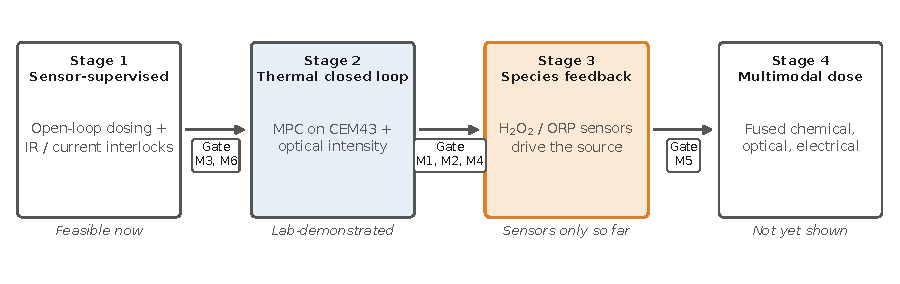
\includegraphics[width=\textwidth]{Fig3_roadmap.pdf}
\caption{Staged roadmap to closed-loop CAP: four stages and three gates. Gates refer to the metrics M1--M6 in Table~\ref{tab:metrics}; Stage~3 (highlighted) is the current bottleneck.}
\label{fig:roadmap}
\end{figure}

\subsection{Research priorities}

\begin{enumerate}
\item Plasma-hardened RONS sensors with antifouling surfaces, reference channels and in-treatment recalibration.
\item Same-device, same-model comparisons of open- and closed-loop CAP reporting M1--M6.
\item Co-integrated hardware that isolates kilovolt drive from microvolt sensor front-ends on one flexible substrate.
\item Fault-tolerant control that detects sensor dropout or bias and falls back to a safe state.
\item Closed-loop regulation of plasma-activated carriers, where loading can be measured before delivery.
\end{enumerate}

\subsection{Conclusions}

Closed-loop CAP is credible in principle and demonstrated in parts. Control is ready: constrained MPC already holds thermal dose and plasma intensity within safety limits in the laboratory. Sensing is not: RONS sensors drift, foul and lose selectivity under plasma exposure, and few devices integrate sensing, control and actuation. The in-silico case study puts numbers on this asymmetry. Feedback removed most of the dose error caused by plant variability, cutting the median CEM43 error from 89\% to 17\% and safety violations from 32\% to 0.1\% of treatments, but the remaining error followed sensor bias and lag, and a degraded sensor roughly tripled it. Progress toward reproducible CAP dosing therefore depends less on new control algorithms than on plasma-hardened sensors, shared benchmark metrics and same-device comparative studies.

%% ---------------------------------------------------------------------------
\section*{CRediT authorship contribution statement}
\textbf{M. Nisha Angeline:} Conceptualization, Methodology, Software, Formal analysis, Investigation, Visualization, Writing -- original draft, Writing -- review \& editing. [Add co-authors and their roles before submission.]

\section*{Funding}
This research did not receive any specific grant from funding agencies in the public, commercial or not-for-profit sectors. [Edit if funded.]

\section*{Declaration of competing interest}
The author declares no known competing financial interests or personal relationships that could have appeared to influence the work reported in this paper.

\section*{Data availability}
No new experimental data were generated. The Monte Carlo simulation script, its fixed random seed (2026) and full numerical output are provided as Supplementary Material S1 and will be deposited in a public repository (Zenodo, DOI to be added) on acceptance.

\section*{Ethics statement}
Not applicable; no human or animal subjects were involved.

\section*{Declaration of generative AI and AI-assisted technologies in the manuscript preparation process}
During the preparation of this work the author used LeapSpace (Elsevier) to generate an initial literature evidence map, and Claude (Anthropic) to verify references, draft and edit text, write the simulation and figure code, and typeset the manuscript. After using these tools, the author reviewed and edited the content, re-checked every cited source and the simulation, and takes full responsibility for the content of the published article.

\section*{Acknowledgements}
[Optional: department, laboratory or colleagues.]

\bibliographystyle{elsarticle-harv}
\bibliography{references}

\end{document}
